\documentclass[ENG]{TFUOC}%IB: CASTELLÀ, CAT: CATALÀ, ENG: ANGLÈS

%%%%%%%%%%%%%%%%%%%%%%%%%%%%%%%%%%%%%%%%%%%%%%%%%%%%%%%%%%%%%%%%%%%%%%%%%%%
% Additional packages
%%%%%%%%%%%%%%%%%%%%%%%%%%%%%%%%%%%%%%%%%%%%%%%%%%%%%%%%%%%%%%%%%%%%%%%%%%%
\usepackage{amsmath}
\usepackage{booktabs}
\usepackage{tabularx}
\usepackage{float}
\usepackage{enumitem}
\usepackage{tikz}
\usetikzlibrary{positioning,arrows.meta,fit,calc,babel}

% Mark for data the student still has to complete or confirm.
% Once everything is reviewed, it can be emptied: \newcommand{\pendent}[1]{#1}
\newcommand{\pendent}[1]{\textcolor{red}{#1}}
% Note for sections not yet written (remove when they are filled in)
\newcommand{\perfer}[1]{\par\noindent\textcolor{gray}{\itshape\small #1}\par}

%%%%%%%%%%%%%%%%%%%%%%%%%%%%%%%%%%%%%%%%%%%%%%%%%%%%%%%%%%%%%%%%%%%%%%%%%%%
% Thesis data
%%%%%%%%%%%%%%%%%%%%%%%%%%%%%%%%%%%%%%%%%%%%%%%%%%%%%%%%%%%%%%%%%%%%%%%%%%%
\title{Emulation of electric guitar distortion with neural networks}
\titcrt{Guitar distortion with neural networks} %Short title for the header
\author{Valentí Ubach Martínez}
\date{November 2026}

\nomPDC{Ismael Benito Altamirano}
\nomPRA{David Masip Rodó}
\titulac{University Master's Degree in Data Science}
\area{Data Science}
\idioma{English}
\credits{\pendent{XX}}
\parcla{guitar amplifier emulation, neural networks, black-box modelling}

\licenc{ccByNcSa}
%Possible licences: ccByNcNd, ccByNcSa, ccByNc, ccByNd, ccBySa, ccBy, GNU, copyright

%%%%%%%%%%
% Abstract in the thesis language (not shown in ENG mode)
\abstractidioma{
Distortion is a defining element of the electric guitar sound. It is traditionally produced by analogue amplifiers and pedals, and reproducing it digitally requires simulating the circuit of each device. This Master's Thesis approaches the problem from a data science perspective: the effect is treated as a \emph{black box} and its behaviour is learned with neural networks from paired recordings of clean and distorted guitar.

The work will create its own dataset, train and compare several neural models (LSTM and GRU networks of different sizes) and evaluate them with objective metrics on unseen data. The goal is to determine which model reproduces the distortion most faithfully and how much data is needed to train it.
}

% Abstract in English.
\abstractenglish{
Distortion is a defining element of the electric guitar sound. It is traditionally produced by analogue amplifiers and pedals, and reproducing it digitally requires simulating the circuit of each device. This Master's Thesis approaches the problem from a data science perspective: the effect is treated as a \emph{black box} and its behaviour is learned with neural networks from paired recordings of clean and distorted guitar.

The work will create its own dataset, train and compare several neural models (LSTM and GRU networks of different sizes) and evaluate them with objective metrics on unseen data. The goal is to determine which model reproduces the distortion most faithfully and how much data is needed to train it.
}

\begin{document}

\estructura

\tableofcontents

\listoffigures

\listoftables

%%%%%%%%%%%%%%%%%%%%%%%%%%%%%%%%%%%%%%%%%%%%%%%%%%%%%%%%%%%%%%%%%%%%%%%%%%%
\chapter{Introduction}
%%%%%%%%%%%%%%%%%%%%%%%%%%%%%%%%%%%%%%%%%%%%%%%%%%%%%%%%%%%%%%%%%%%%%%%%%%%

\section{Context and justification}

Distortion is one of the defining features of the electric guitar sound. It occurs when the instrument signal passes through a nonlinear system (an overdriven valve stage, a diode pedal or a solid-state preamplifier) that alters its waveform, adds harmonics and compresses its dynamics. This behaviour depends on the amplitude and also on the recent history of the signal, which makes it a nonlinear dynamic system that is hard to model~\cite{pakarinen2009}.

Traditionally, distortion has been reproduced digitally by simulating the circuit of each device, a task that requires a great deal of expertise and engineering work~\cite{pakarinen2009,vanhatalo2022}. In recent years, neural networks have made an alternative possible: learning the behaviour of the device directly from data, that is, from pairs of clean and distorted guitar recordings. With this \emph{black-box} approach, emulations have been achieved that are hard to tell apart from the original in listening tests~\cite{wright2019,wright2020}, and today it is the technology behind several commercial products and open-source tools~\cite{nam}.

From a data science point of view, the problem is a complete case of supervised learning on time series: it covers data capture, preprocessing, and the training, evaluation and comparison of models. It is of interest to audio processing research, to the music technology industry and to musicians, who can access the sound of expensive or unavailable equipment with a computer and an audio interface.

As a starting point, a simple prototype has already been built: guitar was recorded in REAPER together with the clean signal and the output of an amplifier simulator plugin, and an LSTM network was trained with PyTorch~\cite{paszke2019} that generates distorted guitar from the clean signal. The prototype shows that the idea is feasible, but it has not been rigorously evaluated: the error was only measured on the training data and the model was not compared with any alternative. This thesis aims to take that step.

\section{Personal motivation}

The motivation for this work comes from the intersection of two of my interests: music and programming applied to data analysis and artificial intelligence. As a student of the master's programme, I am drawn to the possibility of using neural networks to emulate how a guitar amplifier works, a problem I know well as a musician. It also appeals to me because it lets me go through every phase of a data science project with a result that can be \emph{heard}: generating the data myself, training models and checking, by listening to them, whether they work.

\section{Objectives}

\subsection{Hypothesis}

\textit{A small recurrent neural network, trained with a few minutes of audio recorded at home, can faithfully reproduce the distortion of an amplifier simulator on data it has not seen during training.}

\subsection{Specific objectives}

\begin{enumerate}[nosep,label=\textbf{O\arabic*.}]
    \item Create a dataset of clean and distorted guitar, properly aligned and split into training, validation and test sets.
    \item Train several neural models (at least LSTM and GRU networks of different sizes) with a reproducible process.
    \item Evaluate them with objective metrics on unseen data and compare them.
\end{enumerate}

These objectives translate into the following research questions:
\begin{itemize}[nosep]
    \item \textbf{RQ1.} How much data is needed for the model to generalise?
    \item \textbf{RQ2.} Which model architecture and size best reproduce the distortion?
\end{itemize}

\subsection{Scope}



\section{Sustainability, ethical-social and diversity impact}
\label{s:etic}

This section analyses the work according to the three dimensions of the UOC Ethical and Global Commitment competence (CCEG) and its relationship with the Sustainable Development Goals (SDGs)~\cite{onu2015}.

\paragraph{Sustainability.} Training deep learning models consumes energy~\cite{strubell2019}. In this work the impact is low because the models and the data are small, and it will be reduced further by favouring compact models and limiting the number of experiments. In addition, a virtual amplifier can replace part of the physical equipment, which contributes to \textbf{SDG 12} (responsible consumption and production).

\paragraph{Ethical behaviour and social responsibility.} The main ethical risk is \emph{intellectual property}: black-box modelling can reproduce the sound of commercial equipment. For this reason, the models will be used for academic purposes only and no models imitating commercial products will be distributed. The code will be published under an open licence, in line with \textbf{SDG 4} (quality education) and \textbf{SDG 9} (industry, innovation and infrastructure).

\paragraph{Data protection.} The data are audio recordings of the instrument made by the student and contain no personal data, so neither the General Data Protection Regulation~\cite{rgpd2016} nor the UOC Ethics Protocol template needs to be applied. If a listening test with participants were carried out later, the protocol would be completed beforehand.

\section{Approach and method}

\subsection{Research strategy}

Following Oates' classification~\cite{oates2006}, the work combines two research strategies:
\begin{itemize}[nosep]
    \item \textbf{Design and creation}, to build the artefacts: the dataset and the models.
    \item \textbf{Experiment}, to answer the research questions by comparing models trained under controlled conditions.
\end{itemize}
The data generation methods will be \textbf{document-based research}, for the state of the art, and the generation of \textbf{quantitative} data from the experiments. The main metric will be the ESR (\emph{error-to-signal ratio})~\cite{wright2019}:
\begin{equation}
\label{eq:esr}
\mathrm{ESR} = \frac{\sum_{n}\big(y[n]-\hat{y}[n]\big)^2}{\sum_{n} y[n]^2},
\end{equation}
where $y$ is the actual output of the device and $\hat{y}$ the model prediction. The computation time of the models will also be measured.

The planned tools are REAPER for capture and Python, with PyTorch~\cite{paszke2019}, NumPy and Matplotlib, for training and analysis.

\subsection{Work methodology}

Three strategies were considered: (1) using an existing tool such as Neural Amp Modeler~\cite{nam}, which would be fast but would hide the design decisions; (2) reproducing a published work with its data~\cite{wright2020}, which would leave out the capture of our own data; and (3) evolving our own prototype into a systematic study. The third was chosen because it covers the whole data science process, from capture to the presentation of results, and builds on the work already done.

Development will follow an \textbf{iterative, prototype-based} methodology: each iteration (aligned with the continuous assessment activities, PEC) produces an evaluable result that guides the next one. The resources needed are a computer with a GPU, an audio interface, an electric guitar and the software mentioned above, all of which are already available.

\section{Brief summary of products obtained}

\section{Brief description of the remaining chapters}

%%%%%%%%%%%%%%%%%%%%%%%%%%%%%%%%%%%%%%%%%%%%%%%%%%%%%%%%%%%%%%%%%%%%%%%%%%%
% Chapter 2
%%%%%%%%%%%%%%%%%%%%%%%%%%%%%%%%%%%%%%%%%%%%%%%%%%%%%%%%%%%%%%%%%%%%%%%%%%%
%%%%%%%%%%%%%%%%%%%%%%%%%%%%%%%%%%%%%%%%%%%%%%%%%%%%%%%%%%%%%%%%%%%%%%%%%%%
\chapter{State of the art}
\label{c:estat}
%%%%%%%%%%%%%%%%%%%%%%%%%%%%%%%%%%%%%%%%%%%%%%%%%%%%%%%%%%%%%%%%%%%%%%%%%%%

This chapter reviews how the digital emulation of guitar distortion has been approached so far, with an emphasis on data-driven methods. It begins by describing how the review was carried out (Section~\ref{s:revisio}) and the characteristics of the system to be modelled (Section~\ref{s:distorsio}). It then presents the classic modelling families (Section~\ref{s:va}) and, in more detail, neural models (Section~\ref{s:neural}), loss functions and evaluation metrics (Section~\ref{s:avaluacio}), training data (Section~\ref{s:dades}), real-time execution (Section~\ref{s:tempsreal}) and the solutions available on the market (Section~\ref{s:mercat}). It ends with a synthesis of the gaps identified and how this thesis is positioned with respect to them (Section~\ref{s:sintesi}).

\section{Review methodology}
\label{s:revisio}

Following Oates~\cite{oates2006}, the state of the art was produced with a literature survey strategy that uses document-based research as the data generation method. The search was carried out in three steps:
\begin{enumerate}[nosep]
    \item \textbf{Starting point.} Two reference reviews~\cite{pakarinen2009,vanhatalo2022} were used to identify the main authors, groups and conferences in the field.
    \item \textbf{Systematic search.} Google Scholar, Web of Science, IEEE Xplore, arXiv and the archive of the DAFx (\emph{Digital Audio Effects}) conference were searched with combinations of the keywords \emph{guitar amplifier modelling}, \emph{distortion}, \emph{virtual analog}, \emph{black-box}, \emph{neural network}, \emph{LSTM}, \emph{WaveNet}, \emph{real-time} and \emph{audio effects}.
    \item \textbf{Snowballing.} The references and citations of the most relevant works were followed, especially those of the acoustics group at Aalto University and the Centre for Digital Music at Queen Mary University of London.
\end{enumerate}
Peer-reviewed journal and conference articles from the last ten years were prioritised, without excluding earlier foundational works. Preprints (arXiv), software and manufacturers' web pages were used only to describe tools and products, or very recent results not yet published in a journal.

\section{Guitar distortion as a nonlinear system with memory}
\label{s:distorsio}

The signal chain of a distorted electric guitar usually consists of one or more effects pedals, the preamplifier, the power stage, the output transformer and the speaker cabinet~\cite{pakarinen2009}. Distortion appears when one of these elements operates outside its linear region: the diodes of an \emph{overdrive} pedal that clip the signal, the valves of a high-gain preamplifier, or the saturation of the power stage. From a signal processing point of view, this system has three properties that make it hard to model~\cite{pakarinen2009,yeh2009}:
\begin{itemize}[nosep]
    \item \textbf{Nonlinearity.} The output is not proportional to the input: harmonics and intermodulation products appear, and the result depends strongly on the signal level.
    \item \textbf{Memory.} The capacitors and filters of the circuit (for example, the tone stack) make the output depend on past input. Some phenomena, such as the power supply voltage drop (\emph{sag}), have time constants of tens of milliseconds.
    \item \textbf{Aliasing.} Because the nonlinearity creates harmonics above the Nyquist frequency, a naive digital implementation folds them back into the audible band. Oversampling is used to avoid this, which increases the computational cost.
\end{itemize}
These properties explain why a memoryless model (a simple static transfer function) is not enough, and why the system must be treated as a nonlinear dynamic system.

Depending on where and how saturation occurs, several types of distortion are usually distinguished~\cite{pakarinen2009,yeh2009}:
\begin{itemize}[nosep]
    \item \textbf{\emph{Overdrive}}: soft clipping, typically with diodes in the feedback loop of an operational amplifier. The signal saturates gradually and retains part of the dynamics of the performance.
    \item \textbf{Distortion}: hard clipping, typically with diodes connected to ground. The result is more compressed and rich in harmonics.
    \item \textbf{\emph{Fuzz}}: extreme transistor saturation, with biasing effects that depend on the recent signal level and therefore have long memory.
    \item \textbf{Amplifier distortion}: saturation of the valve stages of the preamplifier and the power stage, combined with the frequency response of the tone stack and the transformer.
\end{itemize}
As an illustration, soft and hard clipping can be approximated without memory by functions such as $y=\tanh(g\,x)$ and $y=\max(-1,\min(1,g\,x))$, where $g$ is the gain. Real devices, however, surround these nonlinearities with filters and stateful elements, and this is what data-driven models have to learn.

\section{Virtual analogue audio modelling}
\label{s:va}

The digital emulation of analogue audio equipment is called \emph{virtual analogue modelling}. Techniques are usually classified according to how much knowledge of the circuit they use~\cite{pakarinen2009,vanhatalo2022}. Figure~\ref{fig:taxonomia} summarises the taxonomy, which is used to organise the rest of the chapter.

\begin{figure}[!htbp]
\centering
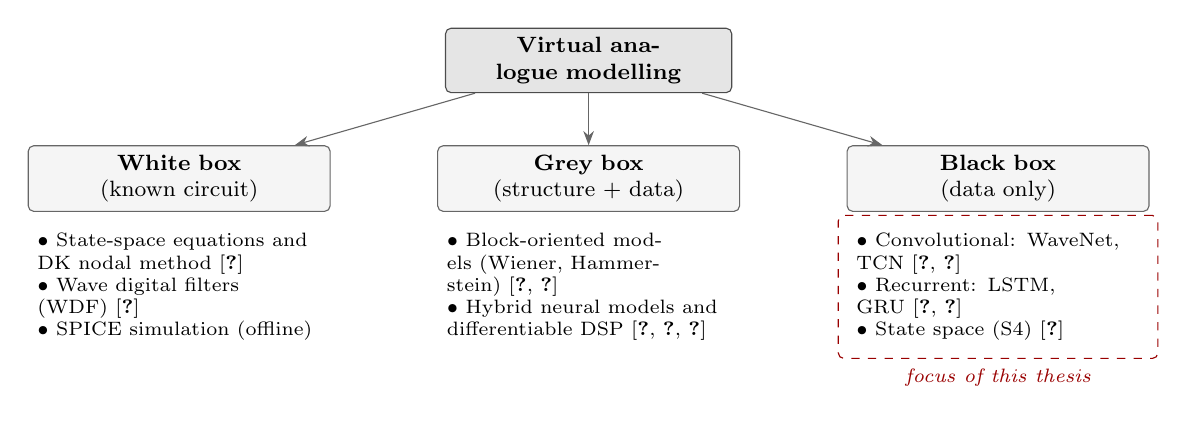
\begin{tikzpicture}[
    font=\footnotesize,
    root/.style={draw=black!70, fill=black!10, rounded corners=2pt, align=center, minimum height=0.8cm, text width=3.4cm},
    cat/.style={draw=black!60, fill=black!4, rounded corners=2pt, align=center, minimum height=0.8cm, text width=3.6cm},
    leaf/.style={align=left, text width=3.6cm, font=\scriptsize},
    arr/.style={-{Stealth[length=1.8mm]}, black!60}]
\node[root] (r) at (0,0) {\textbf{Virtual analogue modelling}};
\node[cat] (w) at (-5.2,-1.5) {\textbf{White box}\\(known circuit)};
\node[cat] (g) at (0,-1.5) {\textbf{Grey box}\\(structure + data)};
\node[cat] (b) at (5.2,-1.5) {\textbf{Black box}\\(data only)};
\draw[arr] (r) -- (w); \draw[arr] (r) -- (g); \draw[arr] (r) -- (b);
\node[leaf, below=0.15cm of w] (wl) {$\bullet$ State-space equations and DK nodal method~\cite{yeh2010}\\$\bullet$ Wave digital filters (WDF)~\cite{werner2015}\\$\bullet$ SPICE simulation (offline)};
\node[leaf, below=0.15cm of g] (gl) {$\bullet$ Block-oriented models (Wiener, Hammerstein)~\cite{eichas2017,novak2010}\\$\bullet$ Hybrid neural models and differentiable DSP~\cite{parker2019,miklanek2023,yeh2024ddsp}};
\node[leaf, below=0.15cm of b] (bl) {$\bullet$ Convolutional: WaveNet, TCN~\cite{damskagg2019,steinmetz2022}\\$\bullet$ Recurrent: LSTM, GRU~\cite{wright2019,wright2020}\\$\bullet$ State space (S4)~\cite{comunita2025}};
\node[draw=red!60!black, dashed, rounded corners=2pt, fit=(bl), inner sep=3pt, label={[font=\scriptsize\itshape, text=red!60!black]below:focus of this thesis}] {};
\end{tikzpicture}
\caption{Taxonomy of virtual analogue modelling techniques.}
\label{fig:taxonomia}
\end{figure}

\subsection{White-box modelling}

White-box models start from the circuit schematic and the physical models of each component (resistors, capacitors, diodes, transistors and valves). From there, they set up the system of differential equations and solve it numerically. Two families stand out in audio. The first is the state-space formulation generated automatically from nodal analysis, the so-called DK method, which Yeh \emph{et al.} applied to pedals and valve amplifiers~\cite{yeh2009,yeh2010}. The second is wave digital filters (WDF), which preserve the modular structure of the circuit and have been extended to arbitrary topologies~\cite{werner2015}.

The main advantage of these models is their fidelity and interpretability: each parameter corresponds to a real component and the controls of the device are reproduced naturally. The drawbacks are that the schematic and component values must be known, that modelling valves is complex and that the computational cost grows quickly with the number of nonlinear elements~\cite{pakarinen2009}. In practice, this makes them hard to scale to many different devices.

\subsection{Grey-box modelling}

Grey-box models combine a simplified structure inspired by the circuit with parameters fitted from measurements. The most common are \emph{block-oriented models}, which chain linear filters and static nonlinear functions: a filter followed by a nonlinearity (Wiener model), a nonlinearity followed by a filter (Hammerstein model) or a combination of both. Eichas \emph{et al.} applied this structure to guitar amplifiers, fitting its parameters with iterative optimisation from measurements of the real device~\cite{eichas2017}. Specific measurement signals have been proposed to identify these models, such as the exponential swept sine, which makes it possible to separate the contribution of each harmonic~\cite{novak2010}.

These models are compact and efficient, but their expressive power is limited by the chosen structure: behaviours that do not fit the cascade of blocks (for example, state dependencies such as \emph{sag}) are hard to capture.

\subsection{Black-box modelling}

Black-box models learn the relationship between the input and the output of the system without using any information about the circuit. For a long time, classic methods of this kind required too many parameters to represent strong distortion~\cite{pakarinen2009,schmitz2018}. Neural networks have overcome this limitation: they are universal approximators whose cost can be controlled by fixing the model size, and they are trained with standard optimisation methods. The next section analyses their variants.

\section{Neural models for distortion emulation}
\label{s:neural}

In a few years, neural emulation has gone from being a research topic to being the technology behind many commercial products~\cite{vanhatalo2022}. The common formulation is a supervised learning problem: given the input sequence $x[n]$ (clean signal) and the output sequence $y[n]$ (signal processed by the device), a network $f_\theta$ is trained so that $\hat{y}[n]=f_\theta(x[n], x[n-1], \dots)$ minimises a loss function. Architectures differ mainly in how they represent the memory of the system.

\subsection{Convolutional models}

The first high-quality results were obtained with convolutional networks inspired by WaveNet~\cite{vandenoord2016}, which stack dilated causal convolutions to obtain a long receptive field with few parameters. With $L$ layers of kernel size $k$ and dilations $d_i$, the receptive field is
\begin{equation}
R = 1 + (k-1)\sum_{i=1}^{L} d_i ,
\end{equation}
so that, for example, ten layers with $k=3$ and dilations $1, 2, 4, \dots, 512$ cover 2\,047 samples, about 46\,ms at 44.1\,kHz. The memory of the model is limited by this value. Damskägg \emph{et al.} adapted this architecture to emulate a valve preamplifier, removing the generative part and making the network predict the output sample directly, and evaluated its quality with listening tests~\cite{damskagg2019}. Shortly afterwards, the same group showed that the model could emulate distortion pedals in real time~\cite{damskagg2019smc}.

In parallel, Martínez Ramírez and Reiss proposed end-to-end models based on convolutions and dense layers for nonlinear effects~\cite{martinez2019}. They also compared several architectures on effects of different kinds, including distortion and compressors~\cite{martinez2020}. Later, temporal convolutional networks (TCN) were optimised for real time, with very small models that run on a CPU~\cite{steinmetz2022}. Comunità \emph{et al.} observed that enlarging the receptive field of these networks is not enough for effects with long memory, such as \emph{fuzz} and compressors. They solved this with time-varying feature modulation (TFiLM), which roughly halves the error in the case of \emph{fuzz}~\cite{comunita2023}.

\subsection{Recurrent models}

Recurrent networks maintain an internal state $h[n]$ that summarises the history of the signal, so that memory does not depend on the size of a receptive field. In the most common form for audio emulation, the model processes one sample at a time:
\begin{equation}
h[n] = \mathrm{RNN}\big(x[n],\, h[n-1]\big), \qquad \hat{y}[n] = \mathbf{w}^{\top} h[n] + b + x[n],
\end{equation}
where the last term is a residual connection, so that the network only has to learn the difference between the input and the output (Figure~\ref{fig:rnn}). The LSTM cell~\cite{hochreiter1997} controls the flow of information with three gates (input, forget and output) and an additional cell state. The GRU~\cite{cho2014} uses two (update and reset) and is lighter. With a scalar input and $H$ units, and counting the two bias vectors used by PyTorch, an LSTM layer has $4H^2+12H$ parameters and a GRU $3H^2+9H$. Since the cost per sample is roughly proportional to this number, going from 64 to 32 units reduces the computation to roughly a quarter. For example, two LSTM layers of 64 units add up to about 50\,000 parameters, while a single LSTM of 40 units has about 6\,900.

\begin{figure}[!htbp]
\centering
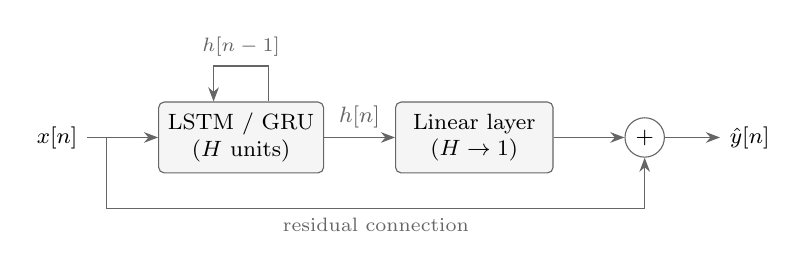
\begin{tikzpicture}[
    font=\footnotesize, node distance=0.9cm,
    blk/.style={draw=black!60, fill=black!4, rounded corners=2pt, minimum height=0.9cm, minimum width=2cm, align=center},
    sum/.style={draw=black!60, circle, inner sep=1pt, minimum size=0.5cm},
    arr/.style={-{Stealth[length=1.8mm]}, black!60}]
\node (x) {$x[n]$};
\node[blk, right=of x] (r) {LSTM / GRU\\($H$ units)};
\node[blk, right=of r] (d) {Linear layer\\($H\rightarrow 1$)};
\node[sum, right=of d] (s) {$+$};
\node[right=0.7cm of s] (y) {$\hat{y}[n]$};
\draw[arr] (x) -- (r); \draw[arr] (r) -- node[above]{$h[n]$} (d); \draw[arr] (d) -- (s); \draw[arr] (s) -- (y);
\draw[arr] (r.north) ++(0.35,0) -- ++(0,0.45) -| node[pos=0.25, above, font=\scriptsize]{$h[n-1]$} ([xshift=-0.35cm]r.north);
\coordinate (xs) at ($(x.east)+(0.25,0)$);
\draw[arr] (xs) -- ++(0,-0.9) -| node[pos=0.25, below, font=\scriptsize]{residual connection} (s.south);
\end{tikzpicture}
\caption{Recurrent model with a residual connection commonly used for distortion emulation~\cite{wright2019}.}
\label{fig:rnn}
\end{figure}

Schmitz and Embrechts were among the first to use an LSTM~\cite{hochreiter1997} to emulate a valve amplifier in real time, with an error below 1\,\% and with the amplifier gain as an additional parameter~\cite{schmitz2018}.

The reference work is that of Wright \emph{et al.}~\cite{wright2019,wright2020}. Its main contributions are:
\begin{itemize}[nosep]
    \item A very simple architecture: a single recurrent layer (LSTM or GRU~\cite{cho2014}) followed by a linear layer, with a residual connection that adds the input to the output.
    \item A training procedure with truncated backpropagation through time and an initial warm-up period for the hidden state, during which the loss is not computed.
    \item The use of the ESR loss with a pre-emphasis filter (Section~\ref{s:avaluacio}).
\end{itemize}
When compared with WaveNet on pedals and amplifiers, recurrent networks achieved similar accuracy at a lower computational cost~\cite{wright2019}. Moreover, in MUSHRA listening tests the best models obtained scores close to those of the hidden reference~\cite{wright2020}.

Later studies have confirmed the validity of the approach. Cassidy and De Sena evaluated LSTM and WaveNet models of a high-gain amplifier (Peavey 6505) with five listening tests. When trained on material from a specific musical genre, the LSTM model was indistinguishable from the real amplifier in ABX tests~\cite{cassidy2023}. Simionato and Fasciani systematically compared several state-based networks and concluded that the LSTM is the best option for distortion and equalisation, although with small differences~\cite{simionato2025}.

This conclusion, however, is not unanimous. In a study with a wide variety of nonlinear effects, Comunità \emph{et al.} found that structured state-space models (S4) with time-varying conditioning gave the best results, and that LSTMs were the least reliable~\cite{comunita2025}. The difference between these studies may be due to the effects considered (\emph{fuzz} and compressors have more memory than an \emph{overdrive}), to the size of the models and to the training procedures. This indicates that the choice of architecture depends on the specific effect and justifies an experimental comparison in each case.

\subsection{Hybrid and neural grey-box models}

An active line of research combines knowledge of the circuit with machine learning to obtain models that are more efficient, more interpretable or that need less data:
\begin{itemize}[nosep]
    \item Parker \emph{et al.} trained deep networks that directly learn the nonlinear state equations of a circuit~\cite{parker2019}. Wilczek \emph{et al.} used neural ordinary differential equations to model diode clipper circuits with fewer parameters and with the ability to change the sampling rate~\cite{wilczek2022}.
    \item Kuznetsov \emph{et al.} showed how to train IIR filters with backpropagation, which makes it possible to integrate classic block-oriented structures into a differentiable model~\cite{kuznetsov2020}.
    \item Miklanek \emph{et al.} combined recurrent networks with nodal analysis of the circuit and obtained amplifier models that need much less training data than a black-box model~\cite{miklanek2023}.
    \item Yeh \emph{et al.} proposed a differentiable digital signal processing (DDSP) model with modules for the preamplifier, the tone stack, the power stage and the transformer. It achieved results comparable to black-box neural models with less than 10\,\% of the operations per sample~\cite{yeh2024ddsp}.
\end{itemize}
Despite these advantages, in the broad comparison by Comunità \emph{et al.} grey-box models still generally fall short of black-box models in accuracy~\cite{comunita2025}.

\subsection{Conditioning on the device controls}

A model trained with a fixed configuration (position of the gain, tone and other controls) only reproduces that configuration, which is why it is called a \emph{capture} or \emph{snapshot}. To reproduce the full range of the device, the model is conditioned on the control values. The simplest way is to concatenate them to the network input~\cite{schmitz2018,wright2020}. More expressive alternatives are feature-wise linear modulation (FiLM)~\cite{comunita2023} and hypernetworks, in which a second network generates the weights of the recurrent network. The latter outperform concatenation on an \emph{overdrive} pedal and on a compressor~\cite{yeh2024hyper}. At industrial scale, Juvela \emph{et al.} (Neural DSP) automated data collection with a robot that turns the amplifier controls, and obtained a conditioned LSTM model that, in listening tests, matches a high-quality SPICE circuit simulation and runs in real time~\cite{juvela2023}.

\subsection{Comparative summary}

Table~\ref{tab:estat} summarises the works most relevant to this thesis.

\begin{table}[H]
\centering
\caption{Summary of the most relevant works on neural emulation of distortion and amplifiers.}
\label{tab:estat}
\scriptsize
\begin{tabularx}{\textwidth}{>{\raggedright\arraybackslash\hsize=0.4\hsize}X>{\raggedright\arraybackslash\hsize=0.95\hsize}X>{\raggedright\arraybackslash\hsize=0.95\hsize}X>{\raggedright\arraybackslash\hsize=1.7\hsize}X}
\toprule
\textbf{Ref.} & \textbf{Architecture} & \textbf{Modelled system} & \textbf{Main contribution} \\
\midrule
\cite{schmitz2018} & LSTM & Valve amplifier & Error $<$1\,\% in real time; gain as an input. \\
\cite{damskagg2019} & WaveNet & Valve preamplifier & First high-quality convolutional model for amplifiers. \\
\cite{wright2019,wright2020} & LSTM, GRU, WaveNet & Pedals and amplifiers & Minimal recurrent architecture, pre-emphasis loss and MUSHRA tests; RNNs match WaveNet at a lower cost. \\
\cite{wright2020percep} & LSTM & Pedals and amplifiers & Pre-emphasis filters in the loss and perceptual improvement. \\
\cite{steinmetz2022} & TCN & Analogue compressor & Very small, efficient TCNs on CPU. \\
\cite{comunita2023} & TCN + TFiLM & \emph{Fuzz} and compressors & Temporal modulation for effects with long memory. \\
\cite{cassidy2023} & LSTM, WaveNet & High-gain amplifier & Genre-specific training; LSTM indistinguishable in ABX. \\
\cite{miklanek2023} & RNN + nodal analysis & Amplifier & Neural grey box with little data. \\
\cite{juvela2023} & Conditioned LSTM & Amplifier (all controls) & Robotic capture; quality equal to SPICE in real time. \\
\cite{yeh2024hyper} & HyperRNN & \emph{Overdrive} and compressor & Hypernetwork conditioning better than concatenation. \\
\cite{yeh2024ddsp} & DDSP & Amplifier & Interpretable model with $<$10\,\% of the operations. \\
\cite{simionato2025} & LSTM, GRU, S4, LRU & Various effects & The LSTM is the best option for distortion. \\
\cite{comunita2025} & LSTM, TCN, GCN, S4, grey box & Various nonlinear effects & S4 with temporal conditioning is the most accurate; LSTM the least reliable. \\
\bottomrule
\end{tabularx}
\end{table}

\section{Loss functions and evaluation}
\label{s:avaluacio}

\subsection{Loss functions}

The most widely used loss function is the \textbf{ESR} (\emph{error-to-signal ratio}), the energy of the error normalised by the energy of the target signal (Equation~\eqref{eq:esr})~\cite{wright2019}. The normalisation makes the error comparable between segments with very different volumes. Wright \emph{et al.} add a term that penalises the difference in the DC component~\cite{wright2020}.

The ESR computed directly on the waveform gives the same weight to all frequencies, whereas the ear is much more sensitive to mid and high frequencies. For this reason, Wright and Välimäki proposed applying a \textbf{pre-emphasis filter} to the output and the target before computing the loss: a first-order high-pass filter of the form $H(z)=1-\alpha z^{-1}$ with $\alpha$ close to 1, or an approximation of A-weighting. Listening tests showed that models trained this way are perceived as more faithful~\cite{wright2020percep}.

An alternative is to compare the signals in the frequency domain. The \textbf{multi-resolution spectral loss} (MR-STFT) computes the difference between the magnitudes of short-time Fourier transforms with several window sizes, so that it captures temporal and frequency detail at the same time~\cite{yamamoto2020}. For each resolution $m$, with $S_m$ the spectrogram magnitude and $N_m$ the number of elements, the loss combines spectral convergence and the difference of log magnitudes:
\begin{equation}
\mathcal{L}_{\mathrm{MR}} = \frac{1}{M}\sum_{m=1}^{M}\left(\frac{\lVert S_m(y)-S_m(\hat{y})\rVert_F}{\lVert S_m(y)\rVert_F} + \frac{1}{N_m}\big\lVert \log S_m(y)-\log S_m(\hat{y})\big\rVert_1\right).
\end{equation}
Since it ignores phase, this loss is usually combined with the ESR, which does take it into account. The \emph{auraloss} library implements these losses for PyTorch~\cite{steinmetz2020}. Finally, Wright \emph{et al.} have explored adversarial training, which even makes it possible to learn from unpaired data~\cite{wright2023}.

\subsection{Objective metrics}

The ESR itself on a test set is the most commonly reported objective metric, and it is often complemented with the spectral error. Other perceptually motivated metrics, such as PEAQ~\cite{itu2001} or the Fréchet Audio Distance (FAD), which compares distributions of embeddings extracted with a pretrained network~\cite{kilgour2019}, are used less often in this field. However, the ESR does not explain all of the perceived quality: two models with a similar ESR can sound different, especially regarding high-frequency artefacts~\cite{wright2020percep}.

\subsection{Perceptual evaluation}

The reference evaluation is listening tests. The \textbf{MUSHRA} method (ITU-R BS.1534) asks participants to rate several stimuli from 0 to 100 against a known reference, including a hidden reference and a low-quality anchor stimulus~\cite{itu2015}. It is the method used by Wright \emph{et al.}~\cite{wright2020}. \textbf{ABX} tests, in which the listener has to identify which of two stimuli matches a third, make it possible to check directly whether a model can be distinguished from the original~\cite{cassidy2023}. Cassidy and De Sena also observed that low-gain passages are the most demanding for distinguishing models~\cite{cassidy2023}, which should be taken into account when choosing the evaluation material.

\section{Training data}
\label{s:dades}

Black-box models need synchronised signal pairs: the clean signal at the device input and the corresponding output. These are usually obtained by sending a previously recorded guitar signal (or a test signal) through the device, a technique known as \emph{reamping}, and recording its output. The critical aspects identified in the literature are:
\begin{itemize}[nosep]
    \item \textbf{Representativeness.} The material must cover the range of levels, frequencies and techniques that will be used. Genre-specific training improves results in that genre~\cite{cassidy2023}.
    \item \textbf{Quantity.} Black-box models are usually trained with a few minutes of audio per configuration. Neural grey-box models reduce this requirement~\cite{miklanek2023}.
    \item \textbf{Alignment and levels.} The latency of the interface and the processors must be compensated, and levels must be calibrated because distortion depends on the input amplitude.
    \item \textbf{Sampling rate.} A model trained at one sampling rate does not work correctly at another without specific adaptations~\cite{carson2024}.
\end{itemize}

To simplify capture, open and commercial tools provide \textbf{standardised training signals} that combine sweeps, noise and guitar passages. This is the case of Neural Amp Modeler~\cite{nam} and of the GuitarML Proteus plugin~\cite{proteus}, which requires a mono file at 44.1\,kHz. As for public datasets, EGFxSet contains 8\,970 guitar notes processed with twelve real effects, including distortion~\cite{pedroza2022}, and ToneTwist AFx collects nonlinear effects for model comparison~\cite{comunita2025}. A recent trend is synthetic data generation: Open-Amp uses hundreds of community-created neural amplifier emulations to generate large-scale, augmented training data~\cite{wright2025openamp}.

\section{Real-time execution}
\label{s:tempsreal}

To use a model live, each audio block (typically 32 to 256 samples) must be processed before the next one arrives. With a block of $N$ samples and a sampling rate $f_s$, the available time is $T=N/f_s$: for example, 2.9\,ms for $N=128$ at 44.1\,kHz. The total input-to-output latency is at least two blocks (one input and one output) plus that of the interface converters, so with $N=128$ it exceeds 5.8\,ms. It is therefore common to characterise a model by its \emph{real-time factor}, the ratio between the computation time and the duration of the processed audio, which must be clearly below 1 to leave headroom for the rest of the system. This imposes three requirements: a low and stable computation time per sample, no memory allocation or locking in the audio thread, and zero or minimal algorithmic latency~\cite{chowdhury2021}. Recurrent models and causal convolutions meet the third requirement because they do not need future samples.

Recurrent networks are evaluated sample by sample, which limits parallelism but makes them very efficient at small sizes. Convolutional networks can take advantage of block processing and vector instructions~\cite{wright2019,steinmetz2022}. The RTNeural library implements LSTM, GRU, convolutional and dense layers with sizes defined at compile time, without dynamic allocation and with several vector computation backends (Eigen, xsimd)~\cite{chowdhury2021}. It is the engine used, for example, by the Proteus plugin~\cite{proteus}.

A specific problem is aliasing. Learned nonlinearities also generate harmonics above the Nyquist frequency. Carson \emph{et al.} have proposed methods for running recurrent networks at sampling rates different from the training one, which enables oversampling~\cite{carson2024}, and specific resampling filters that reduce aliasing in neural distortion models~\cite{carson2025}.

\section{Existing solutions}
\label{s:mercat}

Emulation based on captures of real equipment is well established on the market, and several manufacturers and open projects use neural networks. Some representative examples are:
\begin{itemize}[nosep]
    \item \textbf{Neural DSP Quad Cortex (Neural Capture)}. It learns the behaviour of amplifiers, pedals and cabinets. It offers a version that runs on the device itself and a cloud version with higher resolution for very dynamic equipment such as \emph{fuzz} pedals and compressors~\cite{quadcortex}.
    \item \textbf{Neural Amp Modeler (NAM)}. Open-source software for training and running captures of amplifiers and pedals, based mainly on convolutional networks~\cite{nam}.
    \item \textbf{GuitarML Proteus}. Open-source plugin (GPL-3.0) based on a 40-unit LSTM run with RTNeural, which can also capture the position of one control~\cite{proteus}.
\end{itemize}
Table~\ref{tab:solucions} summarises their main differences.

\begin{table}[H]
\centering
\caption{Comparison of existing neural capture solutions.}
\label{tab:solucions}
\small
\begin{tabularx}{\textwidth}{>{\raggedright\arraybackslash}X>{\raggedright\arraybackslash}X>{\raggedright\arraybackslash}X>{\raggedright\arraybackslash}X}
\toprule
& \textbf{Quad Cortex} & \textbf{NAM} & \textbf{Proteus} \\
\midrule
Type & Commercial hardware & Open-source software & Open-source plugin (GPL-3.0) \\
Model & Not published & Mainly convolutional & 40-unit LSTM \\
Training & On the device or in the cloud & User's computer & Online notebook (Colab) \\
Controls & Fixed capture & Fixed capture & Fixed or one control \\
Execution & Dedicated device & Audio plugin & Plugin with RTNeural \\
\bottomrule
\end{tabularx}
\end{table}

Commercial products do not publish the details of their models. In contrast, NAM and Proteus are open and serve as a direct reference for this work. The size of the Proteus LSTM, for example, is a practical indicator of the size considered sufficient for real use.

\section{Synthesis and positioning of this work}
\label{s:sintesi}

The review leads to the following conclusions:
\begin{enumerate}[nosep]
    \item Black-box neural modelling is the dominant method for capturing distortion equipment and has reached a quality that is hard to tell apart from the original in listening tests~\cite{wright2020,cassidy2023,juvela2023}.
    \item For distortion, small recurrent networks (LSTM, GRU) offer a good trade-off between accuracy and cost~\cite{wright2019,simionato2025}. Even so, there are contradictory results when effects with more memory are included, where S4 models and modulated TCNs are superior~\cite{comunita2023,comunita2025}.
    \item The loss function influences perceived quality, and pre-emphasis is a well-established practice~\cite{wright2020percep}. On the other hand, the correspondence between objective metrics and perception remains an open problem~\cite{wright2020percep,cassidy2023}.
    \item Aliasing and dependence on the sampling rate are recently identified limitations, with solutions still under development~\cite{carson2024,carson2025}.
\end{enumerate}

From this, some \textbf{gaps} are identified where this thesis can provide evidence:
\begin{itemize}[nosep]
    \item \textbf{Low-resource user scenario.} Most studies work with laboratory equipment, curated datasets or, in industry, robotic captures. There is little systematic evidence on how much and what kind of material recorded by a musician at home is needed, and what minimum model size is sufficient in that case.
    \item \textbf{Controlled comparison for distortion.} Conclusions about which architecture is best differ between studies. A comparison with the same data, the same training procedure and the same computational budget, focused on a specific distortion effect, provides useful evidence.
\end{itemize}

This thesis is therefore positioned within black-box modelling with neural networks (Figure~\ref{fig:taxonomia}). It takes the work of Wright \emph{et al.}~\cite{wright2019,wright2020,wright2020percep} as its methodological basis and extends the analysis in the direction of the gaps described. These conclusions justify the objectives set out in Chapter~1.

%%%%%%%%%%%%%%%%%%%%%%%%%%%%%%%%%%%%%%%%%%%%%%%%%%%%%%%%%%%%%%%%%%%%%%%%%%%


%%%%%%%%%%%%%%%%%%%%%%%%%%%%%%%%%%%%%%%%%%%%%%%%%%%%%%%%%%%%%%%%%%%%%%%%%%%
% Remaining chapters (to be completed in the next PECs)
%%%%%%%%%%%%%%%%%%%%%%%%%%%%%%%%%%%%%%%%%%%%%%%%%%%%%%%%%%%%%%%%%%%%%%%%%%%
\chapter{Materials and methods}
\label{c:metodes}

This chapter describes the dataset, the model and the training and evaluation process used in the experiments. All the code was written in Python with PyTorch~\cite{paszke2019}.

\section{Dataset}

\subsection{Capture}

A single electric guitar track was recorded as a direct signal (DI) of 341.3\,s (5\,min 41\,s), at 44.1\,kHz and 24\,bits, with the REAPER digital audio workstation. The track contains an improvisation in which the guitar was played with as many techniques and variations as possible.

From this same track, four outputs were generated by processing it with four different configurations of the Archetype: Plini X amplifier simulator by Neural DSP (digital \emph{reamping}). Each configuration corresponds to a sound with a different amount of distortion:
\begin{itemize}[nosep]
    \item \textbf{acoustic}: clean sound, with very little distortion;
    \item \textbf{crunch}: moderate distortion;
    \item \textbf{dirty\_coil}: moderate distortion, with a different timbral character;
    \item \textbf{high\_gain}: heavy distortion.
\end{itemize}
To avoid effects that a small recurrent network cannot learn (Section~\ref{s:dades}), reverb, delay, modulation effects, stereo effects and the noise gate were disabled. All the outputs therefore share the same input and differ only in the nonlinear processing of the amplifier.

\subsection{Preprocessing}

The files were exported in stereo with the pan shifted to the left, so the left channel is a copy of the right one amplified about 2.4 times and, in some cases, clipped. For this reason only the \textbf{right channel} is used, which is a clean, unclipped copy of the same signal.

Each output was aligned with the input by estimating the processing delay through cross-correlation. The simulator introduces a delay of about 40 samples (close to 1\,ms) in the distorted sounds and of 12 in the clean sound. This delay is not fully compensated: a margin of 25 samples is left uncompensated so that the model, which is causal, does not have to predict future samples (Table~\ref{tab:retards}). Finally, each signal is normalised by dividing it by its peak value.

\begin{table}[H]
\centering
\caption{Measured and compensated delay for each sound (in samples at 44.1\,kHz).}
\label{tab:retards}
\small
\begin{tabular}{lcc}
\toprule
\textbf{Sound} & \textbf{Measured delay} & \textbf{Compensated delay} \\
\midrule
crunch & 40 & 15 \\
dirty\_coil & 39 & 14 \\
acoustic & 12 & 0 \\
high\_gain & 38 & 13 \\
\bottomrule
\end{tabular}
\end{table}

\subsection{Split}

The audio is split in time into three consecutive segments, identical for the four sounds: 70\,\% for training (239\,s), 15\,\% for validation (51\,s) and the final 15\,\% for testing (51\,s). The test set is never used during training.

\section{Model}

An LSTM recurrent network~\cite{hochreiter1997} with two layers of 64 units followed by a linear layer is used, processing the audio sample by sample. To reproduce the four sounds with a single model, the network is \textbf{conditioned}: at each step it receives the guitar sample and a four-component \emph{one-hot} vector indicating which sound it has to generate, similarly to the conditioning on the device controls described in Section~\ref{s:neural}~\cite{wright2020,juvela2023}. The input therefore has five components per step, and the model has about 51\,500 parameters.

\section{Training}

The training audio of the four sounds is cut into consecutive segments of 1024 samples (about 23\,ms), giving 41\,157 segments that are shuffled into batches of 32. Following Wright \emph{et al.}~\cite{wright2019}, the first 256 samples of each segment are excluded from the loss, because the network starts each segment with its internal state set to zero (warm-up). The loss is the ESR (Equation~\eqref{eq:esr}) computed after a first-order pre-emphasis filter $H(z)=1-0.85\,z^{-1}$~\cite{wright2020percep}.

The optimiser is Adam, with a learning rate of 0.001 and the gradient norm clipped to 1. Training runs for a maximum of 200 epochs, with early stopping if the mean validation ESR does not improve for 20 epochs, and the model with the lowest mean validation ESR is kept.

\section{Evaluation}

To evaluate the model, the test set of each sound is processed continuously, keeping the LSTM state between blocks, as in real-time execution. The following are computed:
\begin{itemize}[nosep]
    \item the \textbf{ESR}, unfiltered and with pre-emphasis;
    \item the ESR over 5\,s segments, to detect the hardest passages;
    \item the energy difference per frequency band between the model output and the real output.
\end{itemize}
The model outputs and the real outputs are also saved as audio files so that they can be compared by listening.

\chapter{Results}
\label{c:resultats}

\section{Preliminary experiments with a single sound}

Before the experiment with several sounds, the training process was tuned with a 3-minute recording of a single distorted sound, using the same model. Table~\ref{tab:evolucio} shows how the test ESR evolved with each change. The two changes with the greatest effect were the warm-up and the margin in the delay compensation: without this margin, the model had to predict part of the future and lost a large part of the mid and high harmonics.

\begin{table}[H]
\centering
\caption{Evolution of the test ESR with a single distorted sound.}
\label{tab:evolucio}
\small
\begin{tabularx}{\textwidth}{lXc}
\toprule
\textbf{Version} & \textbf{Change} & \textbf{Test ESR} \\
\midrule
1 & Training/validation/test split and full alignment (20 epochs) & 0.358 \\
2 & 200 epochs & 0.293 \\
3 & 25-sample delay margin and 256-sample warm-up & 0.155 \\
\bottomrule
\end{tabularx}
\end{table}

\section{Conditioned model for four sounds}

Table~\ref{tab:multi} shows the test error of the conditioned model for each sound.

\begin{table}[H]
\centering
\caption{Test error of the conditioned model for each sound.}
\label{tab:multi}
\small
\begin{tabular}{lccc}
\toprule
\textbf{Sound} & \textbf{ESR} & \textbf{Pre-emphasis ESR} & \textbf{Worst 5\,s segment} \\
\midrule
acoustic & 0.028 & 0.149 & 0.09 \\
high\_gain & 0.094 & 0.164 & 0.18 \\
crunch & 0.118 & 0.205 & 0.18 \\
dirty\_coil & 0.179 & 0.272 & 0.29 \\
\midrule
\textbf{Mean} & \textbf{0.105} & \textbf{0.198} & \\
\bottomrule
\end{tabular}
\end{table}

The clean sound (\emph{acoustic}) is, as expected, the one the model reproduces best. Among the distorted sounds, the heavily distorted one (\emph{high\_gain}) obtains a lower error than the moderately distorted ones. A plausible explanation is that heavy distortion strongly compresses the signal and makes it more regular, whereas moderate distortion depends more on the dynamics of the performance. Even so, the three distorted sounds still have a clearly higher error than the clean sound.

By frequency band, between 40\,Hz and 8\,kHz the model output stays within 3\,dB of the real output for all four sounds. Above 8\,kHz, however, the three distorted sounds show an excess of energy of between 14 and 24\,dB, and of about 44\,dB above 16\,kHz. This excess corresponds to high-frequency noise that the original signal does not have. In absolute energy it is small and the ESR barely penalises it, but it is audible. It could be related to the aliasing generated by the learned nonlinearities~\cite{carson2025}.

The mean ESR of the conditioned model (0.105) is lower than the best result obtained with a single sound (0.155). It should be noted, however, that the two experiments do not use the same reference sound or the same amount of data: in the conditioned experiment each sound has about 4\,minutes of training data, twice as much as in the preliminary experiment.

\chapter{Conclusions and future work}

\chapter{Glossary}

%%%%%%%%%%%%%%%%%%%%%%%%%%%%%%%%%%%%%%%%%%%%%%%%%%%%%%%%%%%%%%%%%%%%%%%%%%%
\chapter{Bibliography}
%%%%%%%%%%%%%%%%%%%%%%%%%%%%%%%%%%%%%%%%%%%%%%%%%%%%%%%%%%%%%%%%%%%%%%%%%%%
% Vancouver style: numbered list in order of appearance.
\begingroup
\renewcommand{\chapter}[2]{}% prevents thebibliography from creating a second title
\begin{thebibliography}{99}

\bibitem{pakarinen2009} Pakarinen J, Yeh DT. A review of digital techniques for modeling vacuum-tube guitar amplifiers. \emph{Computer Music Journal}. 2009;33(2):85--100.

\bibitem{vanhatalo2022} Vanhatalo T, Legrand P, Desainte-Catherine M, Hanna P, Brusco A, Pille G, et al. A review of neural network-based emulation of guitar amplifiers. \emph{Applied Sciences}. 2022;12(12):5894.

\bibitem{wright2019} Wright A, Damskägg EP, Välimäki V. Real-time black-box modelling with recurrent neural networks. In: \emph{Proceedings of the 22nd International Conference on Digital Audio Effects (DAFx-19)}. Birmingham; 2019.

\bibitem{wright2020} Wright A, Damskägg EP, Juvela L, Välimäki V. Real-time guitar amplifier emulation with deep learning. \emph{Applied Sciences}. 2020;10(3):766.

\bibitem{nam} Atkinson S. Neural Amp Modeler [software]. GitHub; 2023 [cited 26 Oct 2026]. Available from: \url{https://github.com/sdatkinson/neural-amp-modeler}

\bibitem{paszke2019} Paszke A, Gross S, Massa F, Lerer A, Bradbury J, Chanan G, et al. PyTorch: an imperative style, high-performance deep learning library. In: \emph{Advances in Neural Information Processing Systems 32 (NeurIPS)}. 2019. p.~8024--8035.

\bibitem{onu2015} United Nations. Transforming our world: the 2030 Agenda for Sustainable Development. Resolution A/RES/70/1. New York: UN General Assembly; 2015.

\bibitem{strubell2019} Strubell E, Ganesh A, McCallum A. Energy and policy considerations for deep learning in NLP. In: \emph{Proceedings of the 57th Annual Meeting of the Association for Computational Linguistics (ACL)}. Florence; 2019. p.~3645--3650.

\bibitem{rgpd2016} Regulation (EU) 2016/679 of the European Parliament and of the Council of 27 April 2016 on the protection of natural persons with regard to the processing of personal data and on the free movement of such data (General Data Protection Regulation). \emph{Official Journal of the European Union}. 2016;L119:1--88.

\bibitem{oates2006} Oates BJ. \emph{Researching Information Systems and Computing}. London: SAGE Publications; 2006.

\bibitem{yeh2009} Yeh DT. Digital implementation of musical distortion circuits by analysis and simulation [dissertation]. Stanford (CA): Stanford University; 2009.

\bibitem{yeh2010} Yeh DT, Abel JS, Vladimirescu A, Smith JO. Automated physical modeling of nonlinear audio circuits for real-time audio effects---Part I: theoretical development. \emph{IEEE Transactions on Audio, Speech, and Language Processing}. 2010;18(4):728--737.

\bibitem{werner2015} Werner KJ, Smith JO, Abel JS. Wave digital filter adaptors for arbitrary topologies and multiport linear elements. In: \emph{Proceedings of the 18th International Conference on Digital Audio Effects (DAFx-15)}. Trondheim; 2015.

\bibitem{eichas2017} Eichas F, Möller S, Zölzer U. Block-oriented gray box modeling of guitar amplifiers. In: \emph{Proceedings of the 20th International Conference on Digital Audio Effects (DAFx-17)}. Edinburgh; 2017.

\bibitem{novak2010} Novak A, Simon L, Kadlec F, Lotton P. Nonlinear system identification using exponential swept-sine signal. \emph{IEEE Transactions on Instrumentation and Measurement}. 2010;59(8):2220--2229.

\bibitem{parker2019} Parker JD, Esqueda F, Bergner A. Modelling of nonlinear state-space systems using a deep neural network. In: \emph{Proceedings of the 22nd International Conference on Digital Audio Effects (DAFx-19)}. Birmingham; 2019.

\bibitem{miklanek2023} Miklanek S, Wright A, Välimäki V, Schimmel J. Neural grey-box guitar amplifier modelling with limited data. In: \emph{Proceedings of the 26th International Conference on Digital Audio Effects (DAFx23)}. Copenhagen; 2023.

\bibitem{yeh2024ddsp} Yeh YT, Chen YH, Cheng YC, Wu JT, Fu JJ, Yeh YF, et al. DDSP guitar amp: interpretable guitar amplifier modeling. arXiv:2408.11405 [preprint]. 2024.

\bibitem{damskagg2019} Damskägg EP, Juvela L, Thuillier E, Välimäki V. Deep learning for tube amplifier emulation. In: \emph{Proceedings of the IEEE International Conference on Acoustics, Speech and Signal Processing (ICASSP)}. Brighton; 2019. p.~471--475.

\bibitem{steinmetz2022} Steinmetz CJ, Reiss JD. Efficient neural networks for real-time modeling of analog dynamic range compression. In: \emph{152nd Convention of the Audio Engineering Society}. 2022.

\bibitem{comunita2025} Comunità M, Steinmetz CJ, Reiss JD. Differentiable black-box and gray-box modeling of nonlinear audio effects. \emph{Frontiers in Signal Processing}. 2025;5:1580395. doi:10.3389/frsip.2025.1580395.

\bibitem{schmitz2018} Schmitz T, Embrechts JJ. Real time emulation of parametric guitar tube amplifier with long short term memory neural network. arXiv:1804.07145 [preprint]. 2018.

\bibitem{vandenoord2016} van den Oord A, Dieleman S, Zen H, Simonyan K, Vinyals O, Graves A, et al. WaveNet: a generative model for raw audio. arXiv:1609.03499 [preprint]. 2016.

\bibitem{damskagg2019smc} Damskägg EP, Juvela L, Välimäki V. Real-time modeling of audio distortion circuits with deep learning. In: \emph{Proceedings of the 16th Sound and Music Computing Conference (SMC-19)}. Málaga; 2019.

\bibitem{martinez2019} Martínez Ramírez MA, Reiss JD. Modeling nonlinear audio effects with end-to-end deep neural networks. In: \emph{Proceedings of the IEEE International Conference on Acoustics, Speech and Signal Processing (ICASSP)}. Brighton; 2019. p.~171--175.

\bibitem{martinez2020} Martínez Ramírez MA, Benetos E, Reiss JD. Deep learning for black-box modeling of audio effects. \emph{Applied Sciences}. 2020;10(2):638.

\bibitem{comunita2023} Comunità M, Steinmetz CJ, Phan H, Reiss JD. Modelling black-box audio effects with time-varying feature modulation. In: \emph{Proceedings of the IEEE International Conference on Acoustics, Speech and Signal Processing (ICASSP)}. Rhodes; 2023.

\bibitem{hochreiter1997} Hochreiter S, Schmidhuber J. Long short-term memory. \emph{Neural Computation}. 1997;9(8):1735--1780.

\bibitem{cho2014} Cho K, van Merriënboer B, Gulcehre C, Bahdanau D, Bougares F, Schwenk H, et al. Learning phrase representations using RNN encoder--decoder for statistical machine translation. In: \emph{Proceedings of the Conference on Empirical Methods in Natural Language Processing (EMNLP)}. Doha; 2014. p.~1724--1734.

\bibitem{cassidy2023} Cassidy W, De Sena E. Perceptual evaluation and genre-specific training of deep neural network models of a high-gain guitar amplifier. In: \emph{Proceedings of the 26th International Conference on Digital Audio Effects (DAFx23)}. Copenhagen; 2023.

\bibitem{simionato2025} Simionato R, Fasciani S. Comparative study of state-based neural networks for virtual analog audio effects modeling. \emph{EURASIP Journal on Audio, Speech, and Music Processing}. 2025;2025. doi:10.1186/s13636-025-00416-3.

\bibitem{wilczek2022} Wilczek J, Wright A, Välimäki V, Habets EAP. Virtual analog modeling of distortion circuits using neural ordinary differential equations. In: \emph{Proceedings of the 25th International Conference on Digital Audio Effects (DAFx20in22)}. Vienna; 2022.

\bibitem{kuznetsov2020} Kuznetsov B, Parker JD, Esqueda F. Differentiable IIR filters for machine learning applications. In: \emph{Proceedings of the 23rd International Conference on Digital Audio Effects (DAFx2020)}. Vienna; 2020.

\bibitem{yeh2024hyper} Yeh YT, Hsiao WY, Yang YH. Hyper recurrent neural network: condition mechanisms for black-box audio effect modeling. In: \emph{Proceedings of the 27th International Conference on Digital Audio Effects (DAFx24)}. Guildford; 2024.

\bibitem{juvela2023} Juvela L, Damskägg EP, Peussa A, Mäkinen J, Sherson T, Mimilakis SI, et al. End-to-end amp modeling: from data to controllable guitar amplifier models. In: \emph{Proceedings of the IEEE International Conference on Acoustics, Speech and Signal Processing (ICASSP)}. Rhodes; 2023.

\bibitem{wright2020percep} Wright A, Välimäki V. Perceptual loss function for neural modelling of audio systems. In: \emph{Proceedings of the IEEE International Conference on Acoustics, Speech and Signal Processing (ICASSP)}. Barcelona; 2020.

\bibitem{yamamoto2020} Yamamoto R, Song E, Kim JM. Parallel WaveGAN: a fast waveform generation model based on generative adversarial networks with multi-resolution spectrogram. In: \emph{Proceedings of the IEEE International Conference on Acoustics, Speech and Signal Processing (ICASSP)}. Barcelona; 2020. p.~6199--6203.

\bibitem{steinmetz2020} Steinmetz CJ, Reiss JD. auraloss: audio focused loss functions in PyTorch. In: \emph{Digital Music Research Network One-day Workshop (DMRN+15)}. London; 2020.

\bibitem{wright2023} Wright A, Välimäki V, Juvela L. Adversarial guitar amplifier modelling with unpaired data. In: \emph{Proceedings of the IEEE International Conference on Acoustics, Speech and Signal Processing (ICASSP)}. Rhodes; 2023.

\bibitem{itu2001} International Telecommunication Union. Recommendation ITU-R BS.1387-1: Method for objective measurements of perceived audio quality. Geneva: ITU; 2001.

\bibitem{kilgour2019} Kilgour K, Zuluaga M, Roblek D, Sharifi M. Fréchet Audio Distance: a reference-free metric for evaluating music enhancement algorithms. In: \emph{Proceedings of Interspeech 2019}. Graz; 2019.

\bibitem{itu2015} International Telecommunication Union. Recommendation ITU-R BS.1534-3: Method for the subjective assessment of intermediate quality level of audio systems. Geneva: ITU; 2015.

\bibitem{carson2024} Carson A, Wright A, Chowdhury J, Välimäki V, Bilbao S. Sample rate independent recurrent neural networks for audio effects processing. In: \emph{Proceedings of the 27th International Conference on Digital Audio Effects (DAFx24)}. Guildford; 2024.

\bibitem{proteus} Bloemer K. Proteus [software]. GuitarML; GitHub [cited 26 Oct 2026]. Available from: \url{https://github.com/GuitarML/Proteus}

\bibitem{pedroza2022} Pedroza HE, Meza G, Roman IR. EGFxSet: electric guitar tones processed through real effects of distortion, modulation, delay and reverb. In: \emph{Late-Breaking Demo Session, 23rd International Society for Music Information Retrieval Conference (ISMIR)}. Bengaluru; 2022.

\bibitem{wright2025openamp} Wright A, Carson A, Juvela L. Open-Amp: synthetic data framework for audio effect foundation models. In: \emph{Proceedings of the IEEE International Conference on Acoustics, Speech and Signal Processing (ICASSP)}. Hyderabad; 2025. p.~1--5.

\bibitem{chowdhury2021} Chowdhury J. RTNeural: fast neural inferencing for real-time systems. arXiv:2106.03037 [preprint]. 2021.

\bibitem{carson2025} Carson A, Välimäki V, Wright A, Bilbao S. Resampling filter design for multirate neural audio effect processing. arXiv:2501.18470 [preprint]. 2025.

\bibitem{quadcortex} Neural DSP Technologies. Quad Cortex [Internet]. [cited 26 Oct 2026]. Available from: \url{https://neuraldsp.com/us/quad-cortex}

\end{thebibliography}
\endgroup

\chapter{Annexes}

\end{document}
